\begin{table}[h]
    \caption{Model Arsitektur Client-Server}
    \centering
    \begin{tabular}{c|c|c}
    \hline
    Model - Model Arsitektur\\
    \hline
    Stand-Alone&Client-Server&Multi-Tier\\
    \hline
    \end{tabular}
    \label{1table}
    \end{table}

\section{ArsitekturClientServer
Pada Table \ref{1table} terdapat beberapa model Arsitektur yang terdapat didalam Sebuah Web Service. Arsitektur Client Server merupakan  sebuah model yang membedakan kinerja koputer sebagai client dan server. 
Arsitektur akan menyesuaikan komputer sebagai server dan server akan melayani client yang terhubung kedalam sebuah jaringan.
Server dapat melayani berbagai file server, sebuah printer, bahkan jalur komunikasi.
Client tidak dapat berfungsi sebagai server akan tetapi server dapat berfungsi menjadi client yang dinamakan `server non-dedicated`.
Kerjanga Arsitektur ini sangatlah simpel yaitu server akan menunggu client membuat permintaan dan server akan memproses serta
akan memberikan hasilnya kepada client. Berbeda dengan client, tugas client akan mengirimkan sebuah permintaan kepada server, lalu
client akan menunggu respon yang diberikan oleh server.

\section{PenerapanXMLdiWebService}
Pada layanan web ialah suatu konsep yang baru dalam sistem yang terdistribusi melalui web yang menggunakan teknologi xml dengan menggunakan protokol yang standar SOAP dan HTTP. Dengan menggunakan layanan web sangat dapat mendukung sistem yang terdistribusi yang telah memiliki insfratuktur yang berbeda pula, karena kini layanan web telah menggunakan xml maka dari itu teknologi ini telah dapat mendukung dari berbagai platform yang ada pada sistem maupun aplikasi.

\section{PeranSOAPdiWebSevice}
Pesan berbasis XML melalui jaringan komputer pada program yang berjalan pada sistem operasi, berkomunikasi pada program Operating System yang sama maupun berbeda. 
HTTP dan XML sebagai mekanisme pertukaran data, SOAP dapat berkomunikasi dengan berbagai aplikasi meskipun perbedaan sistem operasi. 
Jadi, SOAP pada web service merupakan aplikasi pesan yang tergantung pada skema XML, sebagai protokol pemaketan pesan-pesan yang digunakan secara bersama oleh aplikasi penggunanya adalah peranan SOAP.

\section{ArsitekturServer}
Arsitektur clien/server menggunakan LAN untuk menjalankan personal komputer, Modul LAN dan DBMS mengendalikan, mengamankan secara bersamaan dan merupakan query untuk support akses dari beberapa pengguna dalam menyambungkan database.
Arsitektur client/memiliki tiga komponen antara :
- Presentation Logic, menangani memformat dan mempresenting data pada pengguna.
- Processing Logic, komponen ini menangani logika data pemrosesan. Proses data logic merupakan aktifitas memvalidasi data, mengindentifikasi proses error pada data.
- Storage Logic, menangani penyimpanan, perbaikan data dari alat penyimpanan yang bekerja dengan aplikasi tersebut.

\section{ArsitekturClient}
Komponen Client sering disebut front-end, sebaliknya komponen server disebut sebagai back-end. 
Komponen Client dijalankan dari sebuah aplikasi dalam workstation dan menerima masukan data dari pengguna, data yang disiapkan dimasukkan oleh pengguna dengan menggunakan teknologi pemroresan lalu mengirimkannya pada komponen server diatas. 
Pada umumnya dalam bentuk request terhadap beberapa service yang dimiliki oleh server. 
Server akan menerima request dari Client dan langsung memprosesnya lalu mengembalikan hasil proses tersebut pada Client dalam sistem server pemrosesan pada DBMS.

\section{Komponen Client-Server}
Dari sisi server bertugas melayani client dalam hal memberikan data yang diminta oleh client.
Lalu, model 2-tier server meyediakan sebuah Stored procedure, Triggers, Query. 
Mengapa menggunakan MySQL dari pada MS SQL server yang lebih kompatibel dengan Visual Basic ? Karena, aplikasi MS SQL bersifat komersial tentu anda harus membelinya. 
Sebaliknya dengan MySQL server bersifat gratis yang mudah didapatkan serta banyak yang menggunakannya. Sedangkan dari sisi Client bertugas menyediakan interface untuk pengguna dalam mengoperasikan pada database. 
Interface dapat dibuat dengan menggunakan bahasa pemrograman yang sudah kita ketahui, contoh seperti bahasa pemrograman pada Visual Studio (VB, C# dan Visual C++), Java, Delpi dan lain-lain. 
Interface menyediakan tampilan untuk memudahkan pengguna dalam mengedit, mendelete serta menampilkan data yang ada di DBMS komputer server ke komputer client.

\section{konsep Client-Server}
Clien-Server ialah komunikasi antara 2 atau lebih pada komputer yang melakukan pembagian tugas masing-masing komputer. Client memiliki beberapa tugas yaitu : input, update, delete, dan dapat menampilkan data sebuah database. Sedangkan Server bertugas untuk menyediakan pelayanan untuk melakukan managemen, yait : menyimpan & mengolah database. Aplkasi Client-server merupakan jawaban atas berkembangnya teknologi informasi, di mana suatu perusahaan memiliki banyak departemen dan harus terhubung satu sama lain dalam melakukan akses data.

\section{Keuntungan Penerapan Client-Server Web Service}
Web Service bisa digunakan untuk alternatif dalam pengembangan Aplikasi n-tier, yang mana dapat dipisahkan
antara Database, aplikasi dan Klien. 

dalam penerapan n-tier ke web service, untuk logika aplikasi dapat diterapkan dengan web services
sehingga disisi klient tidak direpotkan dengan instalasi beberapa layer seperti halnya corba atau sejenisnya.
dengan menggunakan web service, method atau function yang developer buat dapat digunakan berulang - ulang bahkan
untuk keperluan aplikasi yang berbeda (penggunaan kembali function). penerapan yang lebih jauh dari web service adalah SOA dan SOAP

\section{Contoh penerapan Client-server Web Service}
\subsection{Implementasi Web Service Dalam Pencarian Objek Wisata Berbasis Android}
Pengimplementasian dari Web Service didalam sebuah perangkat android untuk memproses
dalam pencarian objek wisata menggunakan android, proses yang terjadi didalamnya adalah :

\begin{enumerate}
    \item Pilihan objek wisata berdasarkan kategori yang diinginkan.
    \item Fitur explore atau pencarian objek wisata berdasarkan kriteria yang diinginkan
    \item Review dan detail mengenai sebuah objek wisata.
    \item Fitur direksi untuk menunjukkan jalan menuju lokasi wisata yang dipilih dengan memanfaatkan google maupun
    \item Add Location atau fitur menambahkan lokasi objek wisata yang dikunjungi
\end{enumerate}

\subsection{Layanan Informasi Pekerjaan Online}
Pada zaman sekarang ini tingkat kebutuhan hidup manusia sudah sangat tinggi sehingga mendorong orang - orang
untuk mencari pekerjaan yang layak agar dapat menghidupi dirinya sendiri dan keluarganya. sehingga 
layanan informasi untuk pencarian pekerjaan secara online dibutuhkan, namun semakin marak juga kebocoran
data dari para pelamar. sehingga dipergunakanlah Web Service yang juga dalam penerapannya menggunakan
implemetasi Client-Server, cara kerja sistem yang ingin dibuat adalah sebagai berikut :

\begin{enumerate}
    \item tamu yang berkunjung untuk mencari pekerjaan 
    \begin{itemize}
        \item mendapatkan lima lowongan pekerjaan terakhir untuk setiap kategori
        \item mencari lowongan kerja berdasarkan kriteria tertentu.
    \end{itemize}
    \item Anggota pencari kerja
    \begin{itemize}
        \item memasukan CV pribadi
        \item memasukan data minat pekerjaan yang diminati
        \item mendapatkan email berisi lowongan kerja yang sesuai data minat pekerajaan
    \end{itemize}
\end{enumerate}

\subsection{Arsitektur Layanan Perawatan Medis terprogram melalui Mobile}
Pada penerapan arsitektur client-server yang satu ini bergerak di bidang kesehatan, dimana Pasien dapat melakukan check kesehatan
walau terpantau jarak yang jauh sekalipun. Dengan menggunakan sebuah telepon selular dapat mencakup kegiatan pengecekan kesehatan.
Dimana Layanan yang diberikan oleh aplikasi ini adalah :
\begin{enumerate}
    \item layanan kesehatan yang menamplkan dengan penggunaan sensor
    \item menjamin dalam sistem keamanannya karena penggunaan software yang dinamik serta dapat diupgrade dengan terpaut data klinik
    \item remote registrasi dimana data yang didapat oleh pasien didapat melalui proses upload dan download yang dilakukan oleh sensor
\end{enumerate}

\section{Arsitektur Database Server}
Dalam Arsitekture Client Server juga membutuhkan atau menggunakan sebuah Database, terutama di dalam server ada yang
dinamakan dengan Arsitekture Database Server yaitu dimana Client akan bertanggung jawab dalam pengelolaan antar muka pemakai
sedangkan Database Server akan bertanggung jawab dengan pada penyimpanan, pengaksesan, serta pemrosesan database.
Di dalam Database Server ini memiliki sebuah kemampuan dalam pemrosesan yang cukup tinggi sehingga beban dalam jaringan akan 
menjadi berkurang. Database Server ini termasuk kedalam two-tier architecture.

\section {Penggunaan Teknologi internet dalam Dunia Bisnis}
Pemasaran internet ada 2 metode yaitu, push dan pull marketing. Keuntungan yang dapat diperoleh dari internet ialah komunikasi global dan interaktif; yang menyediakan suatu informasi dan pelayanan sesuai dengan kebutuhan konsumen; meningkatkan kerjasama; kemudian memungkinkan bagi pengguna untuk membuka pasar,produk, atau pelayanan baru; serta mengintegrasikan aktivitas secara online. 
Pembayaran transaksi electronic commerce diatur oleh Secure Socket Layer yang dikembangkan menjadi Secure Electronic Transaction

\section{Model Arsitektur Client Server}
Dalam Arsitektur Client Server terdapat 3 model arsitektur yaitu :

	\begin{itemize}
	\item Arsitektur Single-tier atau satu lapis
	\item Arsitektur Two-tier atau dua lapis
	\item Arsitektur Three-tier atau tiga lapis
	\end{itemize}

\subsection{Arsitektur Single-tier atau satu lapis}
Pada gambar \ref{1Stand} dijelaskan tentang Arsitektur Single-tier ini merupakan model yang paling sederhana sehingga sangat mudah diginakan oleh pengguna atau user.
Arsitekur Single-tier ini adalah model aristektur yang paling sedikit memiliki alternatif, sehingga dalam Arsitektur Single-tier ini
memiliki kelemahan yaitu seperti kurang aman dan kurang memiliki skalabilitas.

\begin{figure}[ht]
    \centerline{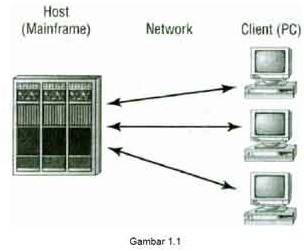
\includegraphics[width=1\textwidth]{figures/2modelstandalone.jpg}}
    \caption{Bahasa Pemrograman yang dipakai di Backend}
    \label{1Stand}
\end{figure}

\subsection{Arsitektur Two-tier atau dua lapis}
Pada gambar \ref{2Tier2} dijelaskan bahwa dalam Arsitektur Two-tier ini dapat dibagi dua dalam pengelolaan informasinya, yaitu dalam UI `User Interface` lingkungan dan dalam
lingkungan server manajemen databasenya. Dibandingkan dengan Arsitektur Single-tier, Arsitekur Two-tier ini mimiliki tingkat
keamanan yang cukup tinggi serta teratur. Arsitektur Two-tier ini memiliki database terpisah pada setiap komputer sehingga dalam
Arsitektur Two-tier ini dapat meningkatkan kinerja dalam keseluruhan situs. Kelemahan yang dimiliki oleh Arsitektur Two-tier ini
adalah tentunya memiliki biaya yang cukup mahal, tidak adanya pembaharuan kode, serta arsitekturnya yang kompleks.

\begin{figure}[ht]
    \centerline{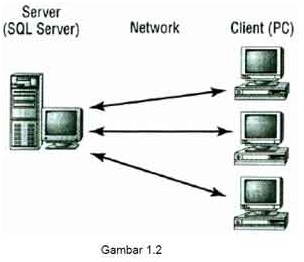
\includegraphics[width=1\textwidth]{figures/2model2tier}}
    \caption{Bahasa Pemrograman yang dipakai di Backend}
    \label{2Tier2}
\end{figure}

\subsection{Arsitektur Three-tier atau tiga lapis}
Awal munculnya Arsitektur Three-tier atau Arsitektur Tiga Lapis ini dikarenakan di Arsitektur sebelumnya memiliki cukup banyak
kelemahannya, maka dari itu Arsitektur Three-tier ini akan mengatasi kelemahan yang dimiliki oleh Arsitektur Two-tier. Kelebihan
dari Arsitektur Three-tier ini yaitu dia memiliki skala yang besar, dan memiliku daya transfer informasi antara web server dengan 
server database optimal, tetapi Arsitektur Three-tier ini juga mempunyai kelemahan atau kekurangan yaitu dengan jumlah tiga lapis
maka biaya yang dikeluarkan cukup mahal, lalu Arsitektur Three-tier ini juga lebih sulit dalam merancang dan mengatur.

\section{RestWebService}
Pada umumnya penemuan yang menyediakan suatu metode dan sistem yang terkomputerisasi untuk memonitori layanan web rest yang termasuk membangkitkan lagi operasi pemanggilan klien layanan web yang berbasis rest yyang akan digunakan untuk memonitoring aktivitas pada layanan web. Metode atau sistem komputerisasi yang lebih lanjut mencakup pemantauan aktivitas layanan web dengan melalui suaru panggilan-panggikan dan tanggapan analisis.

\section {Pemrograman aplikasi pemrograman web pada client server}
Saat ini, perkembangan pada aplikasi yang berbasis Web sangat pesat karena memang memiliki beberapa kelebihan dibandingkan aplikasi berbasis deskop. Berikut adalah beberapa contoh kelebihan pada aplikasi yang berbasis web :
\begin{itemize}
    \item Pada sisi client(pengguna), tidak emerlukan proses intalisasi. Jika terjadi perubahan pada aplikasi, client juga tidak perlu repot-repot melakukan proses update karena cukup dilakukan  pada server.
    \item Data disimpan di sisi server, sehingga akses terhadap data dari sisi client( pengguna) dapat di atur sesuai kebutuhan
    \item Dari sisi client, tidak memerlukan spesifikasi komputer yang besar karena hamper selruh proses aplikasi dilakukan di sisi server
    \item Client(pengguna) lebih aman dari virus atau gangguan keamanan lainnya karena aplikasi berjalan di atas browser.
\end{itemize}


    
